\documentclass[../main.tex]{subfiles}

\begin{document}
\begin{enumerate}[a)]
    \item Para identificar la temperatura potencial, consideramos varias parcelas a lo largo del perfil de temperatura observada, y las hacemos descender por la trayectoria adiabática hasta alcanzar el LCL (NCAA). Luego, las parcelas siguen ascendiendo por el camino adiabático húmedo hasta que dicha trayectoria se vuelve paralela con alguna curva adiabática seca. La curva con la que se vuelve paralela representa la temperatura potencial para cada curva. \\

    Todo esto lo hemos realizado ``a mano'' considerando varios puntos en el gráfico Skew T. A continuación presentamos varias figuras ilustrando el procedimiento realizado.\\

\begin{minipage}{0.5\linewidth}
    \centering
      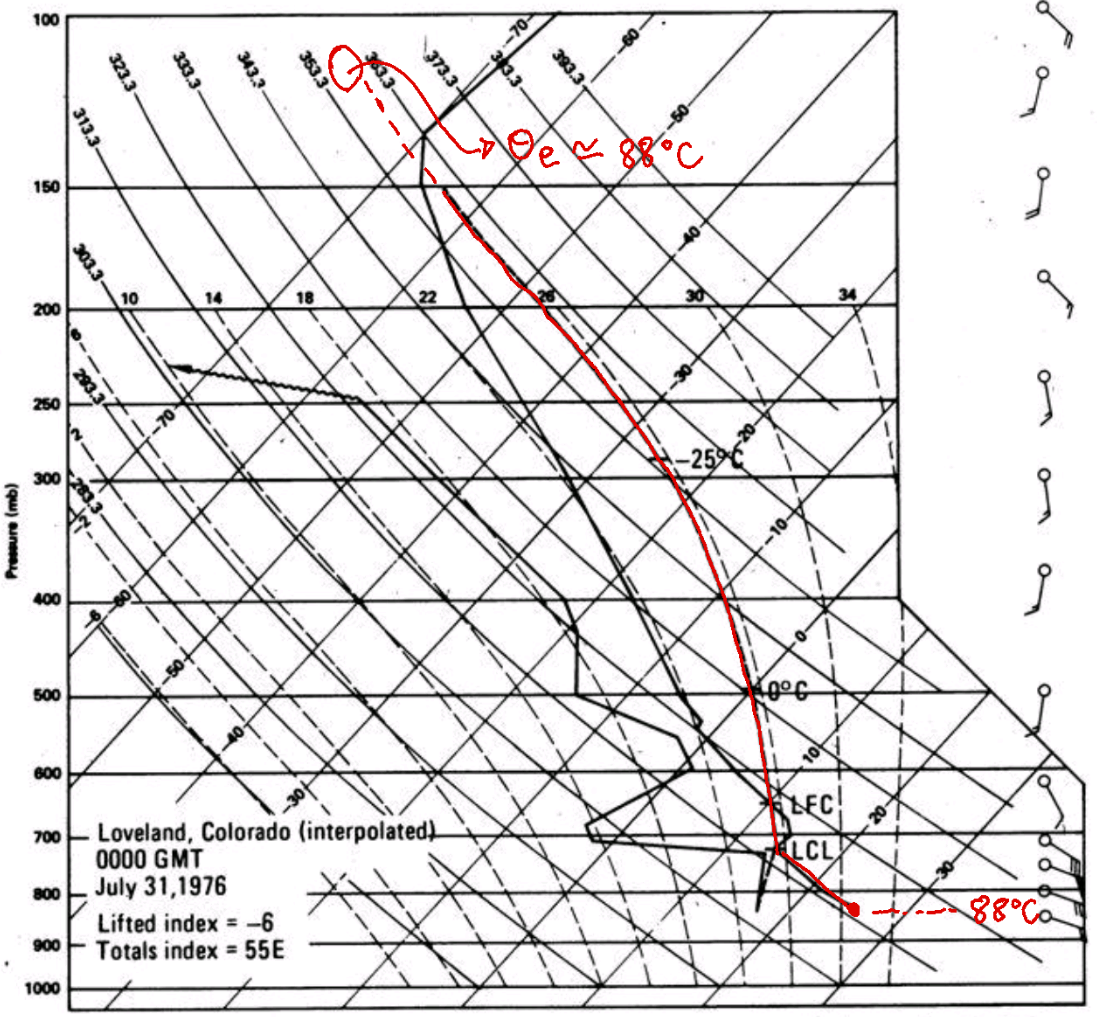
\includegraphics[width=\textwidth]{img/oe1}
\end{minipage}
\begin{minipage}{0.5\linewidth}
    \centering
      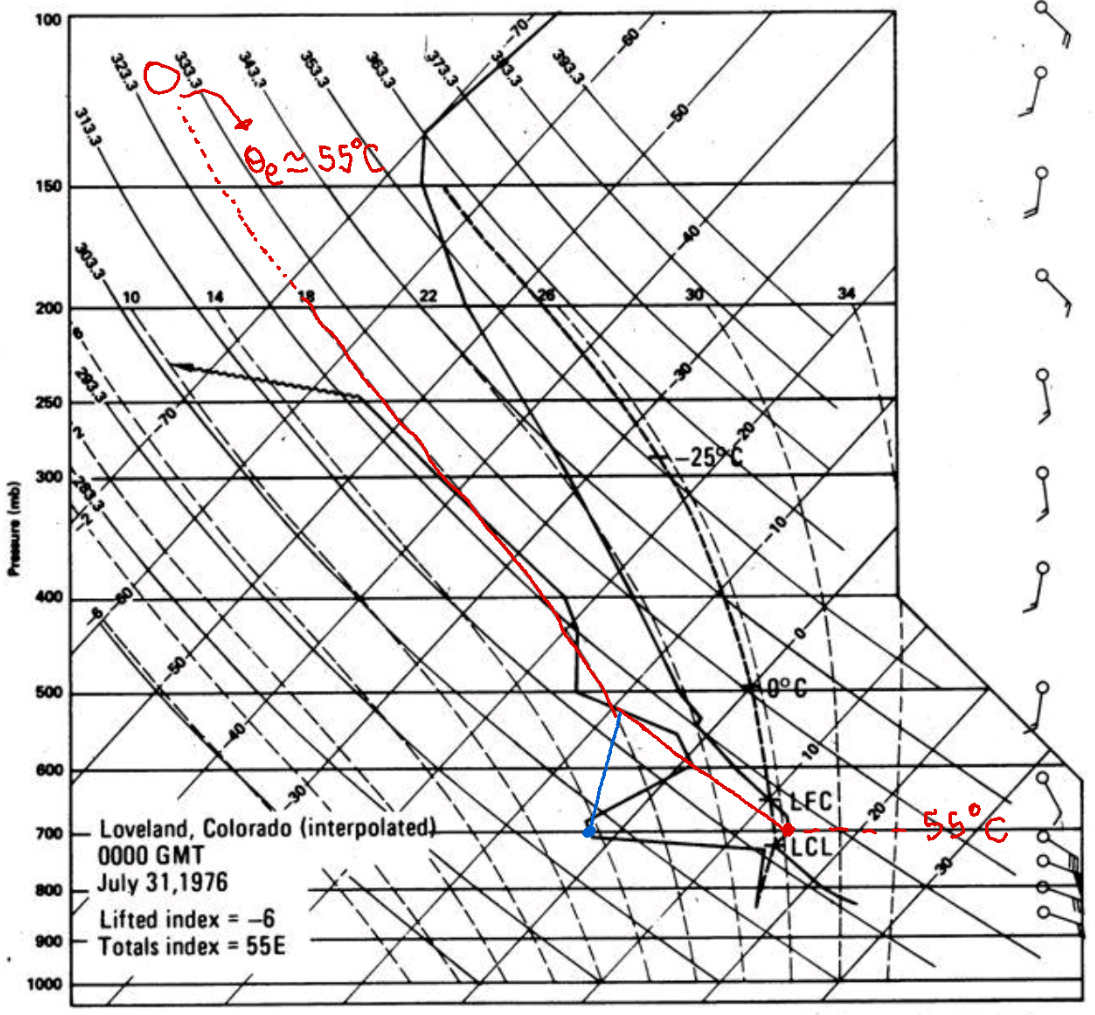
\includegraphics[width=\textwidth]{img/oe2}
\end{minipage}\\


\begin{minipage}{0.5\linewidth}
    \centering
      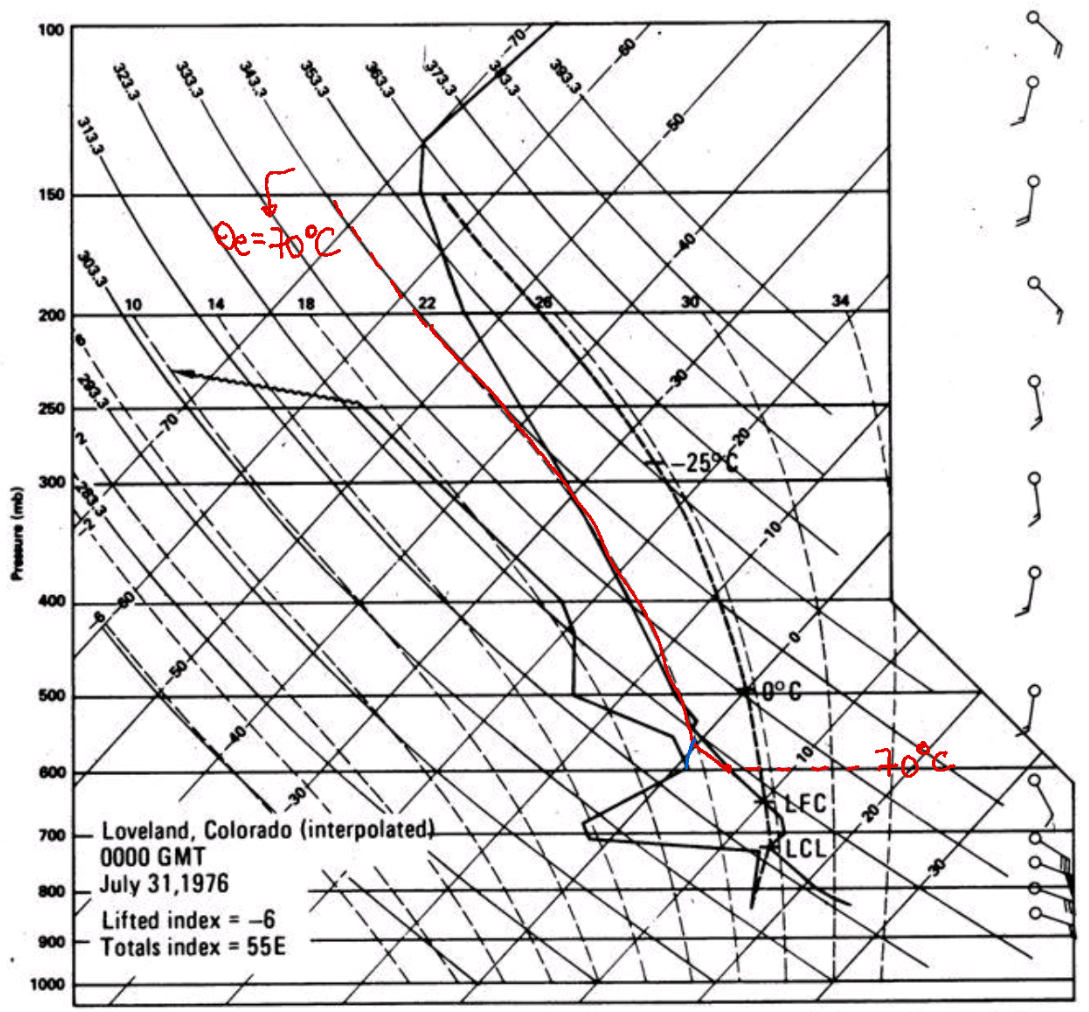
\includegraphics[width=\textwidth]{img/oe3}
\end{minipage}
\begin{minipage}{0.5\linewidth}
    \centering
      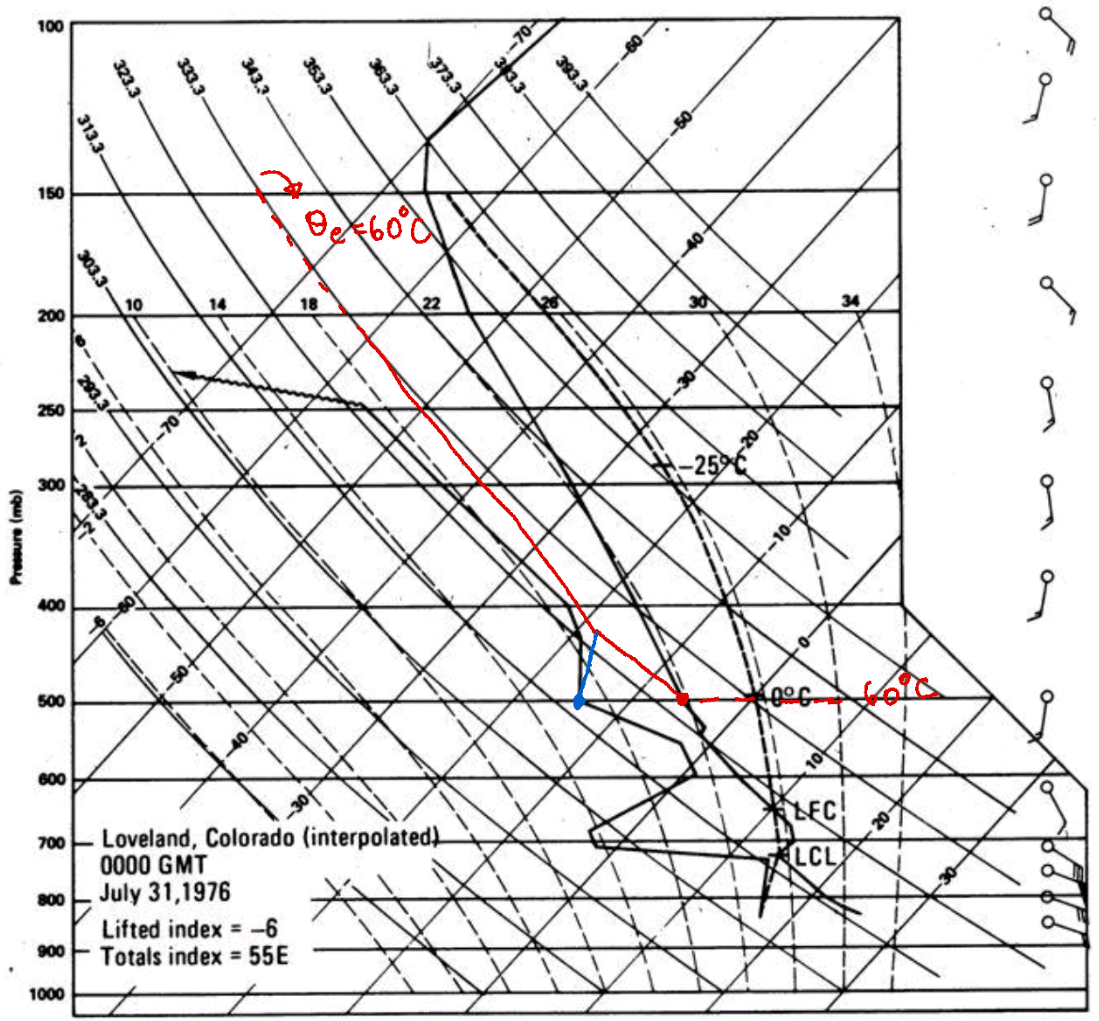
\includegraphics[width=\textwidth]{img/oe4}
\end{minipage}\\

\begin{center}
\begin{minipage}{0.5\linewidth}
      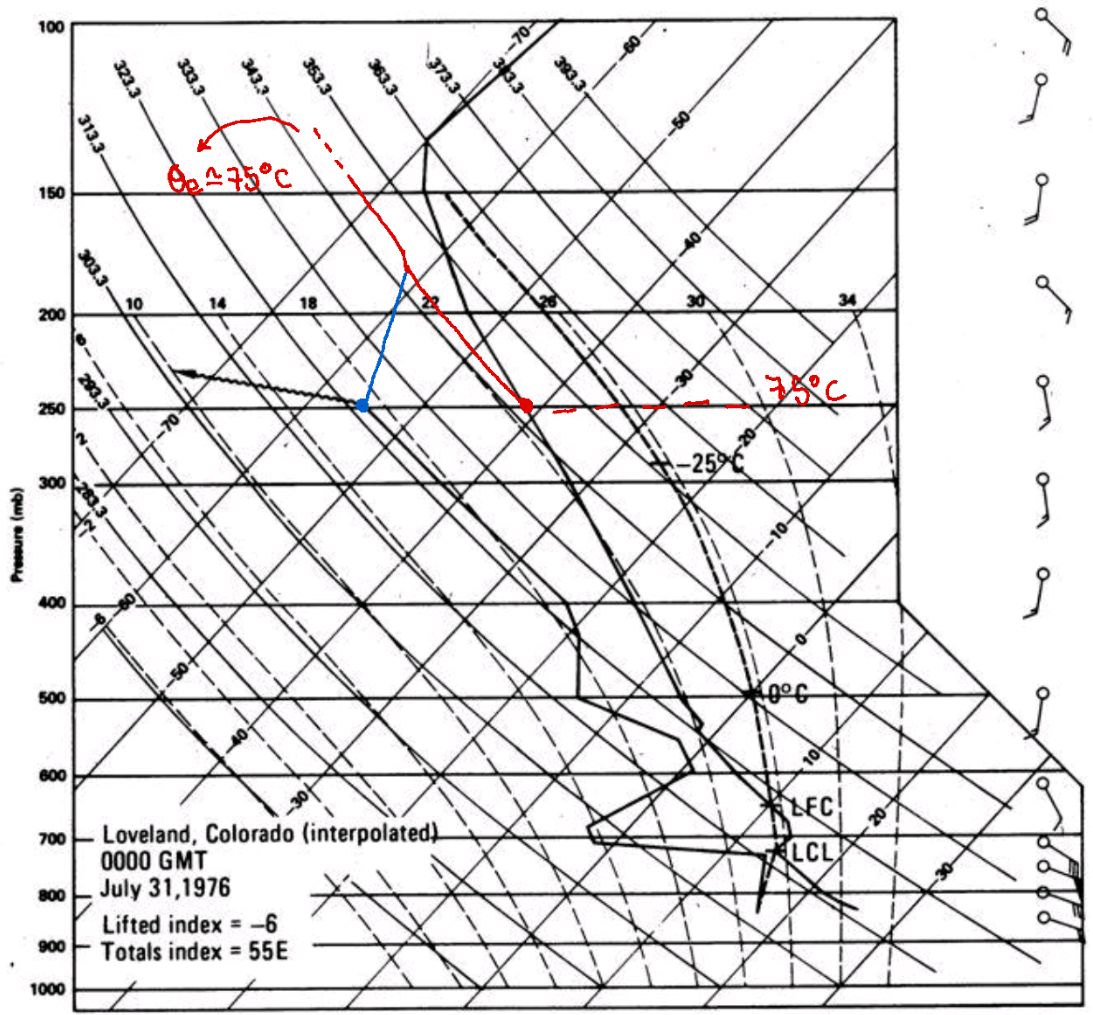
\includegraphics[width=\textwidth]{img/oe6}
\end{minipage}
\end{center}

En las figuras la linea roja es la trayectoria de las parcelas. El segmento azul muestra la linea de razón de mezcla a partir del punto que indica la temperatura punto de rocío. Como en el gráfico no hay líneas de razón de mezcla para guiarnos, hemos estimado la pendiente de estas rectas considerando que debería ser similar al pequeño segmento entre el primer valor de la temperatura punto de rocío y lo que se señala como LCL (el LCL de la parcela de la superficie).\\

Ahora mostraremos todos los valores.\\

\begin{minipage}{\linewidth}
    \centering
        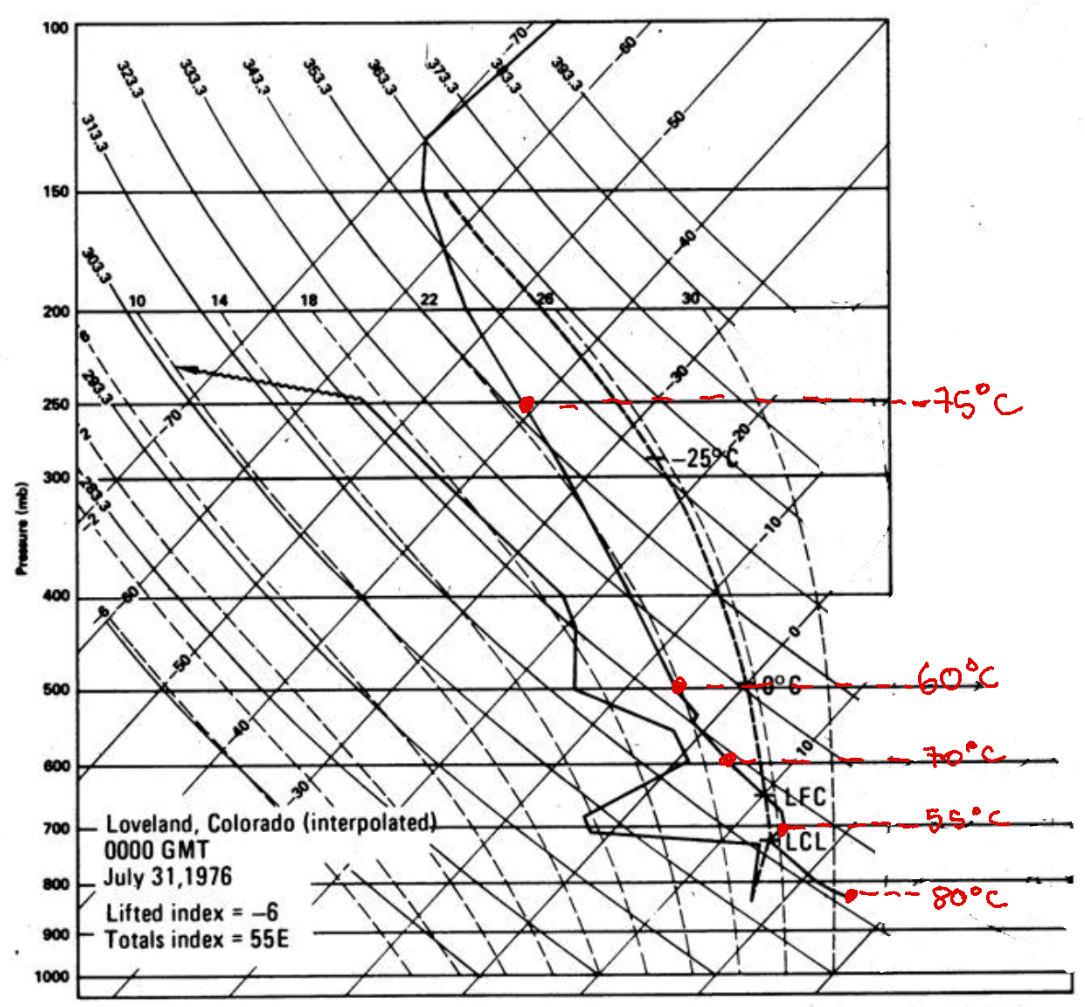
\includegraphics[width=0.6\textwidth]{img/oe_todos}
        \captionof{figure}{Todos los valores obtenidos de temperatura potencial.}
        \label{oes}
\end{minipage}\\

Por simplicidad, en lugar de mostrar los valores de $\theta_e$ respecto a $z$, los mostraremos respecto a la presión, en escala logarítmica.

\begin{minipage}{\linewidth}
    \centering
       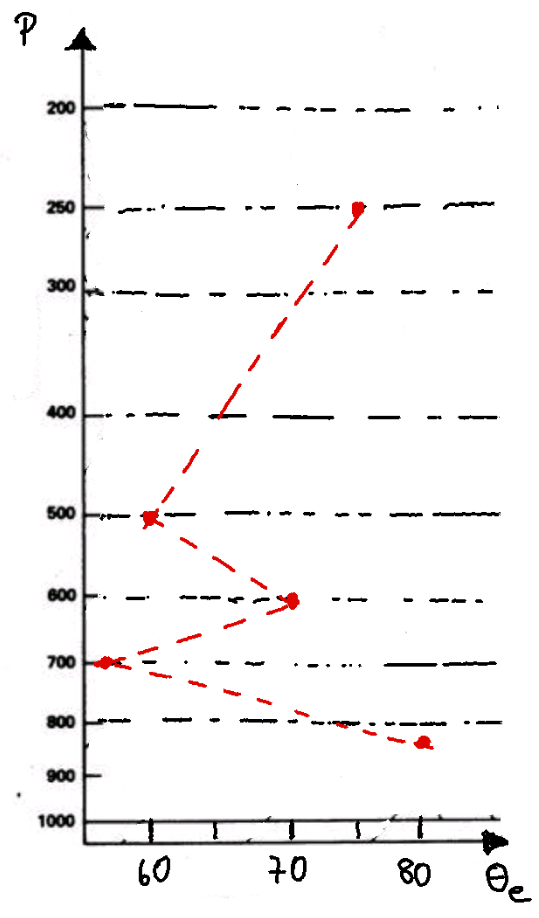
\includegraphics[width=0.3\textwidth]{img/oe_z}
       \captionof{figure}{Perfil vertical de temperatura potencial equivalente. El eje vertical está en términos de la presión en escala logarítmica (en hPa), y el eje horizontal es la temperatura potencial equivalente en grados Celsius.}
       \label{oe_z}
\end{minipage}\\

Para identificar rangos de inestabilidad potencial, verificamos que 
\begin{equation}
    \frac{d\theta_e}{dz} < 0.
\end{equation}
Como $\frac{d}{dz} \simeq \frac{d}{d(\ln P)} $, identificamos que hay inestabilidad potencial en los rangos $(820 \text{ hPa}, 700 \text{ hPa})$ y $(600 \text{ hPa}, 500 \text{ hPa})$.

    \item 


\end{enumerate}
\end{document}
